\begin{figure}[p]
  \centering
  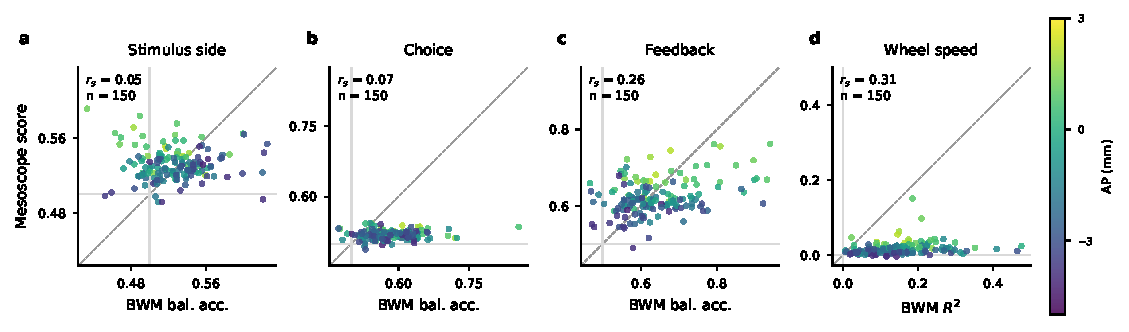
\includegraphics[width=7.00in,height=0.78\textheight,keepaspectratio]{figures/fig5_decoding_n10_scatter/dorsal_decoding_n10_scatter_panels.pdf}
  \caption{Decoding per spatial bin, BWM Neuropixels (x) vs mesoscope (y), decoded from 10 randomly drawn neurons of the session in the bin (mean of 3 draws). Each point is one hexagonal bin (0.4\,mm, hemispheres folded) with at least one session of each modality contributing $\geq$10 neurons; its value is the score averaged across those sessions (same values as the decoding maps). Colour: AP position of the bin. Dashed line: identity; grey lines: chance (0.5 balanced accuracy, 0 for $R^2$). The $p$-values ignore spatial autocorrelation between neighbouring bins and are therefore optimistic. \textbf{a} Stimulus side (Spearman $r_s = 0.05$, $p = 0.55$, 150 bins). \textbf{b} Choice (Spearman $r_s = 0.07$, $p = 0.37$, 150 bins). \textbf{c} Feedback (Spearman $r_s = 0.26$, $p = 0.0013$, 150 bins). \textbf{d} Wheel speed, cross-validated $R^2$ (Spearman $r_s = 0.31$, $p = 9.1\times 10^{-5}$, 150 bins).}
  \label{fig:fig5_decoding_n10_scatter}
\end{figure}
